%%%%%%%%%%%%%%%%%%%%%%%%%%%%%%%%%%%%%%%%%%%%%%%%%%%%%%%%%%%%%%%%%%%%%%%
% 1. Document class
%%%%%%%%%%%%%%%%%%%%%%%%%%%%%%%%%%%%%%%%%%%%%%%%%%%%%%%%%%%%%%%%%%%%%%%

\documentclass[a4paper,12pt]{article}

%%%%%%%%%%%%%%%%%%%%%%%%%%%%%%%%%%%%%%%%%%%%%%%%%%%%%%%%%%%%%%%%%%%%%%%
% 2. Packages
%%%%%%%%%%%%%%%%%%%%%%%%%%%%%%%%%%%%%%%%%%%%%%%%%%%%%%%%%%%%%%%%%%%%%%%

% Tipo de input encoding
\usepackage[utf8]{inputenc}
\usepackage[spanish]{babel}

% Margen del documento
\usepackage[top = 2.5cm, bottom = 2.5cm, left = 2.5cm, right = 2.5cm]{geometry} 

% Para crear tablas
\usepackage{multirow}
\usepackage{booktabs}
\usepackage[table,xcdraw]{xcolor}

% Para manejo de gráficos y figuras
\usepackage{graphicx}
\usepackage{natbib}
\usepackage{float}

% Párrafos
\usepackage{setspace}
%\setlength{\parindent}{0cm}
%\setlength{\parskip}{1em}
%\renewcommand{\baselinestretch}{1.5}

% Cambiar el estilo de las listas
\renewcommand{\labelitemi}{$\bullet$}

% Para crear headers
\usepackage{fancyhdr}

%%%%%%%%%%%%%%%%%%%%%%%%%%%%%%%%%%%%%%%%%%%%%%%%%%%%%%%%%%%%%%%%%%%%%%%
% 3. Header
%%%%%%%%%%%%%%%%%%%%%%%%%%%%%%%%%%%%%%%%%%%%%%%%%%%%%%%%%%%%%%%%%%%%%%%

% Crear el header
\pagestyle{fancy}
\fancyhf{}
\lhead{\footnotesize Trabajo Parcial I: Problema de las Raíces}
\rhead{\footnotesize Grupo 5}

% Colocar el número de la página
\cfoot{\footnotesize \thepage} 

%%%%%%%%%%%%%%%%%%%%%%%%%%%%%%%%%%%%%%%%%%%%%%%%%%%%%%%%%%%%%%%%%%%%%%%
% 4. Title
%%%%%%%%%%%%%%%%%%%%%%%%%%%%%%%%%%%%%%%%%%%%%%%%%%%%%%%%%%%%%%%%%%%%%%%

\begin{document}

\thispagestyle{empty}

% Header de la primera página
\begin{tabular}{p{14cm}}
{\large \bf Análisis Numérico} \\
Pontificia Universidad Javeriana \\ Semestre 2021-10 \\
\hline
% \\
\end{tabular}

% Título
\title{Problema de las raíces: Método Newton-Raphson Relajado y Algoritmo $\Delta^2$ de Aitken}
\author{Alejandro Morales Contreras \\ Carlos Miguel Sánchez Loreto \\ Santiago Vásquez Sánchez}
\date{}

\begingroup
\let\newpage\relax
\maketitle
\endgroup

%%%%%%%%%%%%%%%%%%%%%%%%%%%%%%%%%%%%%%%%%%%%%%%%%%%%%%%%%%%%%%%%%%%%%%%
% 5. Body
%%%%%%%%%%%%%%%%%%%%%%%%%%%%%%%%%%%%%%%%%%%%%%%%%%%%%%%%%%%%%%%%%%%%%%%

\section{Introducción}

%\setlength{\parskip}{1em}

El presente documento pretende mostrar el análisis, implementación y resultados obtenidos del método Newton-Rahpshon Relajado y el Algoritmo $\Delta^2$ de Aitken (Convergencia  Acelerada) para solucionar el problema de las raíces de ecuaciones no lineales. La implementación de los algoritmos fue llevada a cabo en el lenguaje de programación R, y los resultados fueron comparados mediante la herramienta Wolfram Alpha.

%%%%%%%%%%%%%%%%%%%%%%%%%%%%%%%%%%%%%%%%%%%%%%%%%%%%%%%%%%%%%%%%%%%%%%%
% 5.1 Newton-Raphson Relajado
%%%%%%%%%%%%%%%%%%%%%%%%%%%%%%%%%%%%%%%%%%%%%%%%%%%%%%%%%%%%%%%%%%%%%%%

\section{Método Newton-Raphson Relajado}

Es un método iterativo que calcula la raíz de la función $f(x)$ en un intervalo $[a,b]$ basándose en un punto inicial $x_0 \in [a,b]$ que es una buena aproximación de la solución. El método es una ``relajación'' o simplificación del método Newton-Raphson, ya que no calcula la derivada de $f$ en cada iteración, sino que la calcula una única vez, al iniciar el algoritmo.

\subsection{Condiciones de Aplicación del Método}

Para aplicar el método para calcular la raíz de la función $f(x)$ en un intervalo $[a,b]$ con punto inicial $x_0 \in [a,b]$, se deben cumplir las siguientes condiciones:

\begin{enumerate}
    \item $f(x)$ debe ser continua y derivable en el intervalo $[a,b]$
    \item $f(a) \cdotp f(b) < 0$, es decir, existe una raíz para $f(x)$ en $[a,b]$
    \item $f'(x_0) \ne 0$, es decir, la pendiente de $f$ en el punto inicial $x_0$ no es 0
    \item $f''(x_0) \ne 0$, es decir, la función es cóncava o convexa, pero no tiene puntos de inflexión en el punto inicial
    \item Si la pendiente de $f$ en $x_0$ difiere significativamente de la de $f$ cuando $x$ tiende a $f(x)=0$, la convergencia puede ser muy lenta o no existir (el método diverge) 
\end{enumerate}

\newpage

\subsection{Explicación Geométrica}

El método Newton-Raphson Relajado es un método iterativo. Esto quiere decir que para hallar el valor de $x$ en la iteración $i+1$, se debe conocer el valor de $x$ en la iteración $i$, y operar desde este. \par

Para una función $f(x)$ acotada en el intervalo $[a,b]$, con punto inicial $x_0 \in [a,b]$, la fórmula iterativa del método está dada por: \par

\[ x_{n+1} = x_n - \frac{f(x_n)}{f'(x_0)} \]

Visto geométricamente, se puede explicar de la siguiente forma:

% Figura: Explicación geométrica de NRR
\vspace{-1em}
\begin{figure}[h!]
\centering
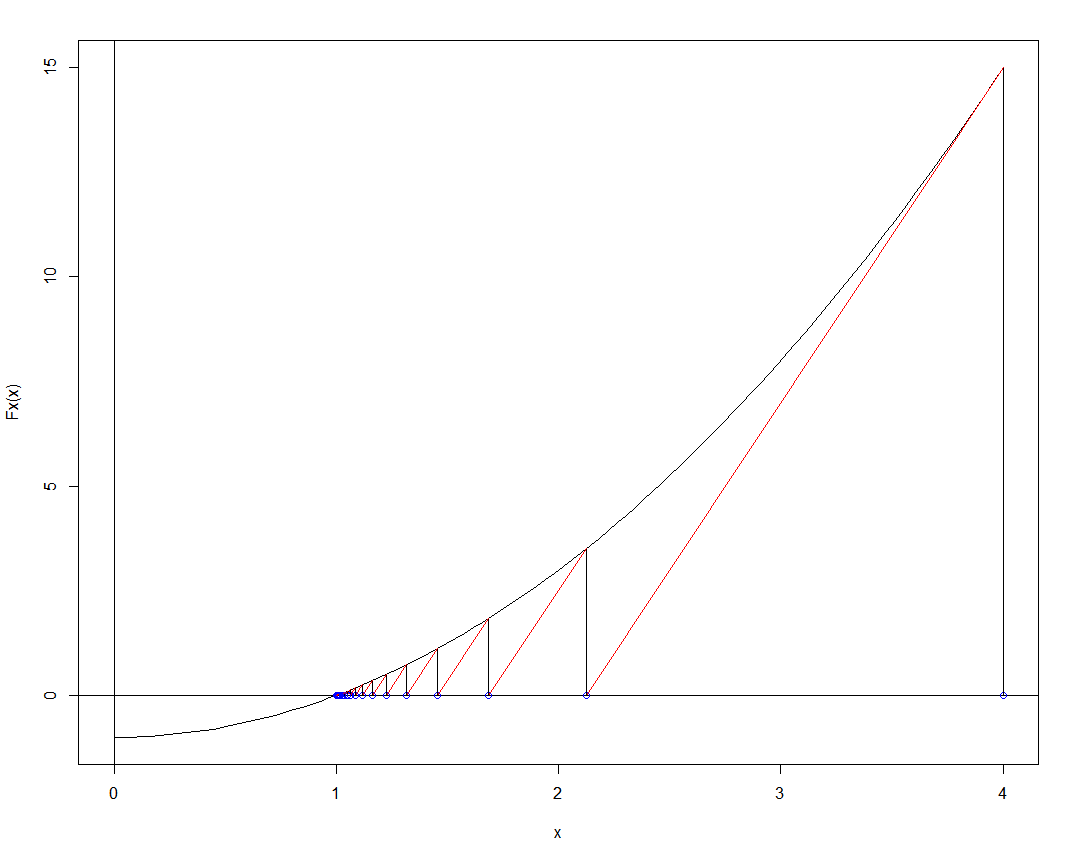
\includegraphics[scale=0.5]{img/explicacion_geometrica.png}
\vspace{-1em}
\caption{Explicación Geométrica del método Newton-Raphson Relajado}
\label{fig:exp_geom_nrr}
\end{figure}

El método consiste en, por cada paso, calcular el corte que existe con el eje horizontal, partiendo desde un $x$, y trazando una recta con pendiente $f'(x_0)$ desde $f(x)$ hacia la horizontal. Cada nuevo corte pasa a ser el $x$ con el cual se calcula el siguiente corte, hasta llegar a la raíz de la función.

\newpage

\subsection{Diagrama de Flujo del Método}

A continuación se presenta el diagrama de flujo que modela cómo se debe implementar el método Newton-Raphson Relajado: \par 

\vspace{1em}

% Figura: Diagrama de flujo NRR
\begin{figure}[h!]
\centering
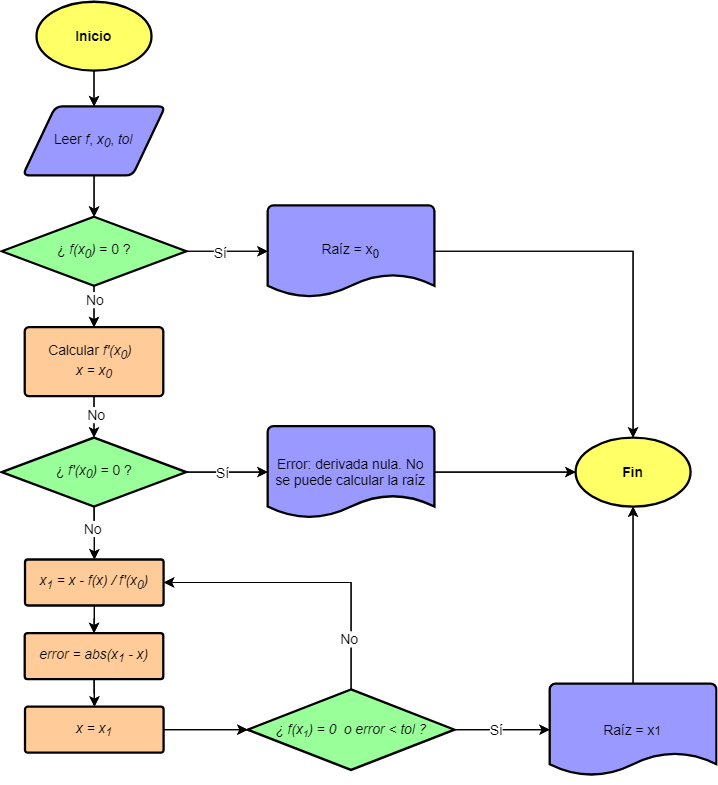
\includegraphics[scale=0.8]{img/flujograma_nrr.png}
\vspace{-1em}
\caption{Diagrama de flujo del método Newton-Raphson Relajado}
\label{fig:flujograma_nrr}
\end{figure}

\newpage

\subsection{Implementación, Resultados Obtenidos y Comportamiento del Método}

El método fue implementado en R. El código fuente puede ser encontrado en el siguiente repositorio: \par

\vspace{1em}
https://github.com/AlejandroMoralesContreras/analisis-numerico.git \par
\vspace{1em}

El problema consistía en aplicar el método para encontrar las raíces de las siguientes funciones, bajo las tolerancias $10^{-8}$, $10^{-16}$, $10^{-32}$, $10^{-56}$. Para resolver el problema a tolerancias altas, se encontró que el épsilon de la máquina ($\epsilon_{maq} \approx 2.22 \times 10^{-16}$) impedía dar una buena aproximación de la respuesta. Por ende, se hizo uso de la librería \emph{Rmpfr} para aumentar la precisión de las operaciones. \par

A continuación se presentan los resultados obtenidos, la cantidad de iteraciones que le toma al método alcanzar dicho resultado, así como la comparación con el valor real: \par

\subsubsection{$f(x)=cos^2(x)-x^2$}

Se toma como punto inicial $x_0 = 1$ \par

\begin{table}[ht!]
\begin{tabular}{clr}
Tol      & \multicolumn{1}{c}{x}                                      & \multicolumn{1}{c}{i} \\
1.00E-08 & 0.73908514                                                 & 10                    \\
1.00E-16 & 0.7390851332151607                                         & 20                    \\
1.00E-32 & 0.73908513321516064165531208767387                         & 39                    \\
1.00E-56 & 0.73908513321516064165531208767387340401341175890075746503 & 66                    \\
Wolfram  & 0.73908513321516064165531208767387340401341175890075746496 &                      
\end{tabular}
\end{table}

\vspace{-1em}
\begin{itemize}
    \item Pérdida de significancia: el algoritmo no tiene una pérdida de significancia relevante (solo los últimos tres dígitos).
    \vspace{-10pt}
    \item Número de iteraciones: el algoritmo demora una cantidad de iteraciones promedio.
    \vspace{-10pt}
    \item Convergencia: el algoritmo converge linealmente.
\end{itemize}

\subsubsection{$f(x)=xsin(x)-1$ en $[-1,2]$}

Se toma como punto inicial $x_0 = 1$ \par

\begin{table}[ht!]
\begin{tabular}{clr}
Tol      & \multicolumn{1}{c}{x}                                     & \multicolumn{1}{c}{i} \\
1.00E-08 & 1.1141571                                                 & 5                     \\
1.00E-16 & 1.114157140871930                                         & 8                     \\
1.00E-32 & 1.1141571408719300873005251781692                         & 15                    \\
1.00E-56 & 1.1141571408719300873005251781692039039541013760493755956 & 25                    \\
Wolfram  & 1.1141571408719300873005251781692039039541013760493755953 & \multicolumn{1}{l}{} 
\end{tabular}
\end{table}

\vspace{-1em}
\begin{itemize}
    \item Pérdida de significancia: el algoritmo no tiene una pérdida de significancia relevante (solo el último dígito).
    \vspace{-10pt}
    \item Número de iteraciones: el algoritmo demora una cantidad de iteraciones menor al promedio.
    \vspace{-10pt}
    \item Convergencia: el algoritmo converge linealmente a una gran razón.
\end{itemize}

\newpage

\subsubsection{$f(x)=x^3-2x^2+\frac{4}{3}x-\frac{8}{27}$}

Se toma como punto inicial $x_0 = 0.6$ \par

\begin{table}[ht!]
\begin{tabular}{clr}
Tol      & \multicolumn{1}{c}{x}                                 & \multicolumn{1}{c}{i} \\
1.00E-08 & 0.6848291                                             & 500                   \\
1.00E-16 & 0.67953959366266881                                   & 1000                  \\
1.00E-32 & 0.675781083128382253910615418135421                   & 2000                  \\
1.00E-56 & 0.673116162063445266916517084609949961304664611816406 & 4000                  \\
Wolfram  & 0.666666666666666666666666666666666666666666666666667 & \multicolumn{1}{l}{} 
\end{tabular}
\end{table}

\vspace{-1em}
\begin{itemize}
    \item Pérdida de significancia: el algoritmo sufre una gran cantidad de pérdida de significancia.
    \vspace{-10pt}
    \item Número de iteraciones: el algoritmo demora una cantidad de iteraciones muy alta. No se estabiliza, y se tuvo que cortar para poder finalizar.
    \vspace{-10pt}
    \item Convergencia: el algoritmo parece converger linealmente, aunque lo hace de manera muy lenta y dificilmente computable.
\end{itemize}

\subsubsection{$f(x)=\frac{668.061}{x} (1 - e^{-0.146843 x}) - 40$}

Se toma como punto inicial $x_0 = 10$ \par

\begin{table}[ht!]
\begin{tabular}{clr}
Tol      & \multicolumn{1}{c}{x}                                     & \multicolumn{1}{c}{i} \\
1.00E-08 & 14.801141                                                 & 18                    \\
1.00E-16 & 14.80114070018228                                         & 35                    \\
1.00E-32 & 14.801140700182285887665341806477                         & 67                    \\
1.00E-56 & 14.801140700182285887665341806477076404804050289002632207 & 111                   \\
Wolfram  & 14.801140700182285887665341806477076404804050289002632208 & \multicolumn{1}{l}{} 
\end{tabular}
\end{table}

\vspace{-1em}
\begin{itemize}
    \item Pérdida de significancia: el algoritmo no tiene una pérdida de significancia relevante (solo el último dígito).
    \vspace{-10pt}
    \item Número de iteraciones: el algoritmo demora una cantidad de iteraciones ligeramente mayor al promedio.
    \vspace{-10pt}
    \item Convergencia: el algoritmo converge linealmente.
\end{itemize}

\subsubsection{$f(x)=x^3-2x-5$}

Se toma como punto inicial $x_0 = 2$ \par

\begin{table}[ht!]
\begin{tabular}{clr}
Tol      & \multicolumn{1}{c}{x}                                    & \multicolumn{1}{c}{i} \\
1.00E-08 & 2.0945515                                                & 9                     \\
1.00E-16 & 2.094551481542326                                        & 17                    \\
1.00E-32 & 2.0945514815423265914823865405793                        & 34                    \\
1.00E-56 & 2.094551481542326591482386540579302963857306105628239179 & 57                    \\
Wolfram  & 2.094551481542326591482386540579302963857306105628239180 & \multicolumn{1}{l}{} 
\end{tabular}
\end{table}

\vspace{-1em}
\begin{itemize}
    \item Pérdida de significancia: Pérdida de significancia: el algoritmo no tiene una pérdida de significancia relevante (solo los últimos dos dígitos).
    \vspace{-10pt}
    \item Número de iteraciones: el algoritmo demora una cantidad de iteraciones promedio.
    \vspace{-10pt}
    \item Convergencia: el algoritmo converge linealmente.
\end{itemize}

\newpage

\subsection{Problema de Significancia}

El método no presentó problemas de significancia relevantes en la mayoría de los casos. Sin embargo, para la función $f(x)=x^3-2x^2+\frac{4}{3}x-\frac{8}{27}$, cuya raíz real es $\frac{2}{3}=0.66666...$, se encontró que al algoritmo le costaba calcular correctamente la solución. Aunque estaba convergiendo hacia el valor, lo hacía de manera muy lenta y muy poco eficiente. Se vió la necesidad de contar con una cantidad de iteraciones máximas para poder analizar una respuesta. \par 

La manera más fácil de remediar este problema sería aplicando el método Newton-Raphson para estos casos, en vez del Relajado. Esto debido a que el método normal permite calcular de nuevo la pendiente de $f$ por cada paso, convergiendo así más rapidamente hacia la respuesta. \par

\subsection{Raíces Múltiples}

El método Newton-Raphson Relajado no es capaz de calcular raíces múltiples de manera simultánea. Siempre dependerá de la cercanía del punto inicial $x_0$ con respecto a la raíz de la función dada. \par

\subsubsection{Multiplicidades}

\begin{table}[ht!]
\begin{tabular}{llr}
\multicolumn{1}{c}{Función}  & 
\multicolumn{1}{c}{M} 
\\
$f(x) = cos^2(x)-x^2$              & 1                        
\\
$f(x) = xsin(x)-1$                 & 1                 
\\
$f(x) = x^3-2x^2+\frac{4}{3}x-\frac{8}{27}$   & 2 
\\
$f(x) = \frac{668.061}{x} (1 - e^{-0.146843 x}) - 40$ & 2
\\
$f(x) = x^3-2x-5$             & 1                         
\end{tabular}
\end{table}

\vspace{-1em}

\subsection{Funciones Pares, Impares y Periódicas}

Según el análisis de los resultados obtenidos, el método no tiene particularidades especiales cuando se trabaja con funciones pares o impares. Ya que el método parte de un punto inicial $x_0$, este se va a dedicar a encontrar la raíz más cercana a este punto. \par

Para el caso de las funciones periódicas, sí se encontró que el método operaba de una manera distinta. Toca ser muy cuidadoso de dar una buena aproximación al valor inicial, sí se desea encontrar la raíz correcta. Se evidenció que si el punto inicial era muy ambiguo, la función podía tender a una raíz que no fuera la más cercana a este. \par

\newpage

\subsection{Relación entre $\varepsilon_i$ y $\varepsilon_{i+1}$} 

\par

\subsubsection{Orden de Convergencia}

El orden de convergencia del método se verifica mediante la fórmula: \par

\[ 0 \leq \lim_{i\to\infty} \frac{|x_{i+1}-x*|}{|x_i-x*|^r} < \infty \]

donde $r$ es el máximo entero positivo que satisface la fórmula, y representa el orden de convergencia. Al hacer los cálculos para cada ejercicio, se encuentra que $r=1$ para todas las soluciones. Esto confirma que el método converge linealmente. \par

\subsubsection{Razón de Convergencia}

La razón de convergencia $S$ se verifica mediante la fórmula: \par

\[ \lim_{i\to\infty} \frac{\varepsilon_{i+1}}{\varepsilon_i} = S < 1\]

En la siguiente tabla se presentan las razones de convergencia obtenidas para cada una de las funciones evaluadas. Se tomó como medida de tolerancia $10^{-56}$. \par

\begin{table}[ht!]
\begin{tabular}{llr}
\multicolumn{1}{c}{Función}                         & \multicolumn{1}{c}{S} & \multicolumn{1}{c}{i} \\
$f(x)=cos^2(x)-x^2$                                 & 0.1496                & 66                    \\
$f(x)=xsin(x)-1$                                    & 0.0051                & 25                    \\
$f(x)=x^3-2x^2+\frac{4}{3}x-\frac{8}{27}$           & 0.9996                & 4000                  \\
$f(x)=\frac{668.061}{x} (1 - e^{-0.146843 x}) - 40$ & 0.3242                & 111                   \\
$f(x)=x^3-2x-5$                                     & 0.1161                & 57                   
\end{tabular}
\end{table}

\vspace{-2em}

\subsubsection{Gráfica de la Relación}

A continuación se presenta la gráfica que relaciona $\varepsilon_i$ con $\varepsilon_{i+1}$ para el método Newton-Raphson Relajado: \par

% Figura: Relación entre Ei y Ei+1
\vspace{-1em}
\begin{figure}[ht!]
\centering
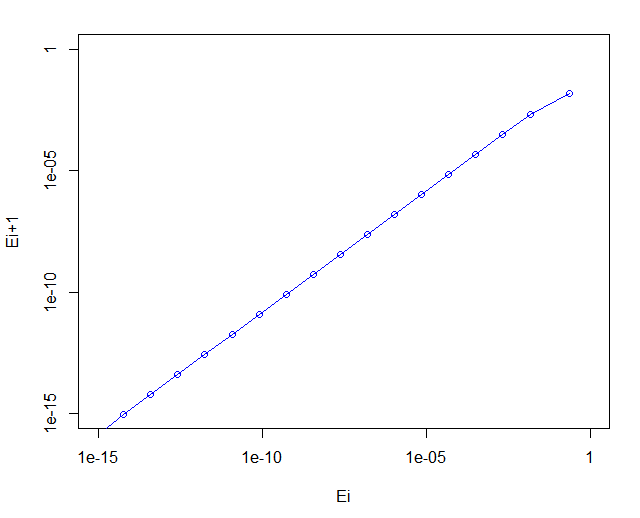
\includegraphics[scale=0.6]{img/relacion_error_nrr.png}
\vspace{-1em}
\caption{Relación entre $\varepsilon_i$ y $\varepsilon_{i+1}$ del método Newton-Raphson Relajado}
\label{fig:relacion_error_nrr}
\end{figure}

\newpage

\subsection{Tolerancia contra Iteraciones}

A continuación se presenta la gráfica que modela la relación entre la cantidad de iteraciones que le toma al método obtener la raíz y el error calculado para esa iteración. El análisis se realizó a partir de la función $f(x)=cos^2(x)-x^2$ con punto inicial $x_0 = 1$. \par

% Figura: Tolerancia contra Iteraciones nrr
\vspace{-1em}
\begin{figure}[ht!]
\centering
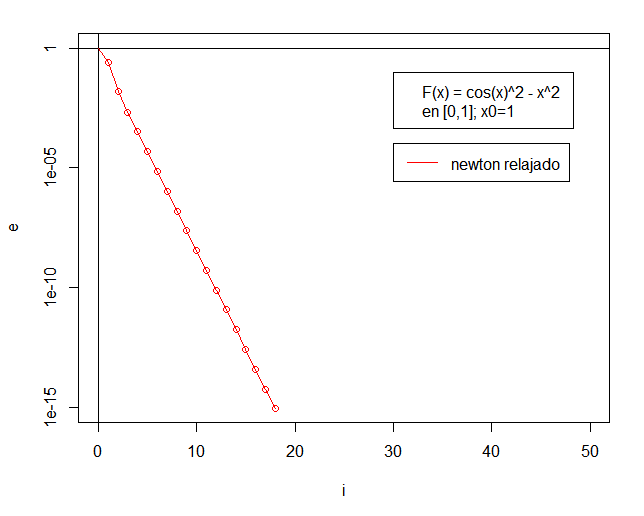
\includegraphics[scale=0.6]{img/tol_i_nrr.png}
\vspace{-1em}
\caption{Tolerancia vs. Iteraciones del método Newton-Raphson Relajado}
\label{fig:tol_i_nrr}
\end{figure}

\vspace{-1em}

\subsection{Comparación del Método contra el de Bisección}

Se encontró que ambos métodos tienen convergencia lineal. Sin embargo, se estableció que el método de Newton-Raphson Relajado es más eficiente, alcanza una mayor tolerancia en menor tiempo, y tiene menor pérdida de significancia a altas tolerancias. \par 

A continuación se presenta la gráfica que compara la convergencia del método Newton-Raphson Relajado contra el método de la bisección. El análisis se realizó a partir de la función $f(x)=cos^2(x)-x^2$ en el intervalo $[0,1]$ con punto inicial $x_0 = 1$. \par

% Figura: NRR vs. Biseccion
\vspace{-1em}
\begin{figure}[ht!]
\centering
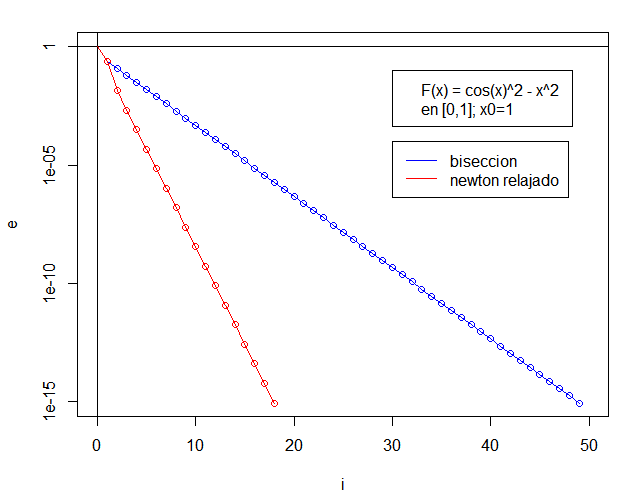
\includegraphics[scale=0.6]{img/nrr_vs_biseccion.png}
\vspace{-1em}
\caption{Método Newton-Raphson Relajado vs. Método de la Bisección}
\label{fig:nrr_biseccion}
\end{figure}

\newpage

\subsection{Comparación del Método contra Taylor}

La comparación entre el método con la solución por series de Taylor demostró que el algoritmo es mucho más preciso que una aproximación polinómica realizada mediante Taylor. \par 

El análisis se realizó para la función $f(x)=cos^2(x)-x^2$ con punto inicial $x_0 = 1$. La serie de Taylor se realizó centrada en $0$, de orden $16$. La herramienta para calcular la serie fue Wolfram Alpha. A continuación se presenta el polinomio obtenido: \par

\[ 1 - 2 x^2 + \frac{x^4}{3} - \frac{2x^6}{45} + \frac{x^8}{315} - \frac{2 x^{10}}{14175} + \frac{2 x^{12}}{467775} - \frac{4x^{14}}{42567525} + \frac{x^{16}}{638512875} + O(x^{18}) \]

La raíz correspondiente a este polinomio es: \par

\begin{table}[ht!]
\begin{tabular}{clc}
\multicolumn{1}{l}{} & \multicolumn{1}{c}{x}              & Tol                  \\
Taylor               & 0.73908513321519627015195351373908 &                      \\
NRR                  & 0.73908513321516064165531208767387 & 1.00E-32             \\
Valor Real           & 0.73908513321516064165531208767387 & \multicolumn{1}{l}{}
\end{tabular}
\end{table}

Como se puede evidenciar, comparando el valor obtenido mediante el método Newton-Raphson Relajado, se determina que el algoritmo es más preciso a la hora de calcular las soluciones.

\newpage

%%%%%%%%%%%%%%%%%%%%%%%%%%%%%%%%%%%%%%%%%%%%%%%%%%%%%%%%%%%%%%%%%%%%%%%
% 5.1 Algoritmo Delta cuadrado de Aitken
%%%%%%%%%%%%%%%%%%%%%%%%%%%%%%%%%%%%%%%%%%%%%%%%%%%%%%%%%%%%%%%%%%%%%%%

\section{Algoritmo $\Delta^2$ de Aitken}

En este apartado consideramos una técnica, llamada Método $\Delta^2$ de Aitken, que se utiliza para acelerar la convergencia de cualquier sucesión que converja linealmente, independientemente de su origen. \par

Supongamos que $p_n$ es una sucesión linealmente convergente con límite $p$. El método $\Delta^2$ de Aitken está basado en la suposición de que la sucesión $\hat{P_n}$ definida por: \par

\[ \hat{P_n} = p_n - \frac{(p_{n+1} - p_n)^2}{p_{n+2} - 2p_{n+1} + p_n} \]

converge más rápidamente a $p$ que la sucesión original $P_n$. \par

\subsection{Condiciones de Aplicación del Método}

Para que el método $\Delta^2$ de Aitken acelerare la convergencia dada una sucesión $P_n$, se deben cumplir las siguientes condiciones: \par

\begin{enumerate}
    \item La sucesión debe converger linealmente, es decir, $\lim_{i \to{+} \infty}{\frac{e_{i+1}}{e_i}}= \lambda $ ;    $0<\lambda<1$.
    \item $i$ es lo suficientemente grande para que el cociente pueda usarse para aproximar el límite.
    \item  Todas las $e_i$ deben tener el mismo signo, es decir, $e_i \times e_{i+1} \ge 0$.
    \item $e_i = p_n - p \ne 0, \forall x \ge 0$.
    
\end{enumerate}

\newpage

\subsection{Diagrama de Flujo del Método}

A continuación se presenta el diagrama de flujo que modela cómo se debe implementar el algoritmo $\Delta^2$ de Aitken: \par 

\vspace{1em}
% Figura: Diagrama de flujo Aitken
\begin{figure}[h!]
\centering
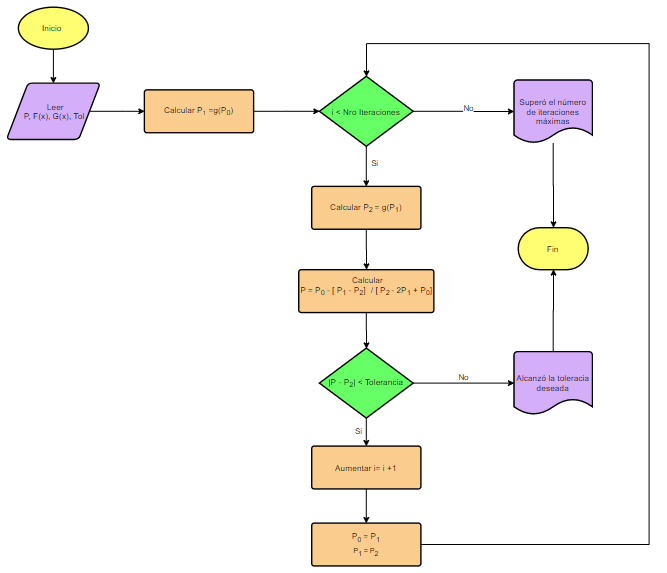
\includegraphics[scale=0.8]{img/Flujograma Aitken.png}
\caption{Diagrama de flujo del método $\Delta^2$ de Aitken}
\label{fig:flujograma_aitken}
\end{figure}

\newpage

\subsection{Implementación, Resultados Obtenidos y Comportamiento del Método}

El método fue implementado en R. El código fuente puede ser encontrado en el siguiente repositorio: \par

\vspace{1em}
https://github.com/AlejandroMoralesContreras/analisis-numerico.git \par
\vspace{1em}

A continuación se presentan los resultados obtenidos, la cantidad de iteraciones que le toma al método alcanzar dicho resultado, así como la comparación con el valor real: \par

\subsubsection{$f(x)=cos^2(x)-x^2$}

Se toma como punto inicial $x_0 = 1$ \par

\begin{table}[ht!]
\begin{tabular}{clr}
Tol      & \multicolumn{1}{c}{x}                                      & \multicolumn{1}{c}{i} \\
1.00E-08 & 0.73908513                                                 & 4                     \\
1.00E-16 & 0.7390851332151606                                         & 5                     \\
1.00E-32 & 0.73908513321516064165531208767387                         & 6                     \\
1.00E-56 & 0.73908513321516064165531208767387340401341175890075746503 & 7                     \\
Wolfram  & 0.73908513321516064165531208767387340401341175890075746496 &                      
\end{tabular}
\end{table}

\vspace{-1em}
\begin{itemize}
    \item Pérdida de significancia: el algoritmo no tiene una pérdida de significancia relevante (solo los últimos tres dígitos).
    \vspace{-10pt}
    \item Número de iteraciones: el algoritmo demora una cantidad de iteraciones eficiente (es muy rápido).
    \vspace{-10pt}
    \item Convergencia: el algoritmo acelera la convergencia lineal.
\end{itemize}

\subsubsection{$f(x)=xsin(x)-1$ en $[-1,2]$}

Se toma como punto inicial $x_0 = 1$ \par

\begin{table}[ht!]
\begin{tabular}{clr}
Tol      & \multicolumn{1}{c}{x}                                     & \multicolumn{1}{c}{i} \\
1.00E-08 & 1.11415714                                                & 4                     \\
1.00E-16 & 1.11415714087193008                                       & 5                     \\
1.00E-32 & 1.114157140871930087300525178169203                       & 6                     \\
1.00E-56 & 1.1141571408719300873005251781692039039541013760493755943 & 8                     \\
Wolfram  & 1.1141571408719300873005251781692039039541013760493755953 &                      
\end{tabular}
\end{table}

\vspace{-1em}
\begin{itemize}
    \item Pérdida de significancia: el algoritmo no tiene una pérdida de significancia relevante (solo los últimos dos digitos).
    \vspace{-10pt}
    \item Número de iteraciones: el algoritmo demora una cantidad de iteraciones eficiente (es muy rápido).
    \vspace{-10pt}
    \item Convergencia: el algoritmo acelera la convergencia lineal.
\end{itemize}

\newpage

\subsubsection{$f(x)=x^3-2x^2+\frac{4}{3}x-\frac{8}{27}$}

Se toma como punto inicial $x_0 = 0.6$ \par

\begin{table}[ht!]
\begin{tabular}{clr}
Tol      & \multicolumn{1}{c}{x}                                 & \multicolumn{1}{c}{i} \\
1.00E-08 & 0.66666987                                            & 32                    \\
1.00E-16 & 0.6666698708192892                                    & 34                    \\
1.00E-32 & 0.66666987081928920008177594108415                    & 35                    \\
1.00E-56 & 0.666669870819289200081775941084153759859569023172871 & 38                    \\
Wolfram  & 0.666666666666666666666666666666666666666666666666667 &                      
\end{tabular}
\end{table}

\vspace{-1em}
\begin{itemize}
    \item Pérdida de significancia: el algoritmo sufre una pérdida de significancia considerable.
    \vspace{-10pt}
    \item Número de iteraciones: el algoritmo demora una cantidad de iteraciones mayor al promedio.
    \vspace{-10pt}
    \item Convergencia: el algoritmo parece acelerar la convergencia lineal. Sin embargo, es más lento de lo normal.
\end{itemize}

\subsubsection{$f(x)=\frac{668.061}{x} (1 - e^{-0.146843 x}) - 40$}

Se toma como punto inicial $x_0 = 10$ \par

\begin{table}[ht!]
\begin{tabular}{clr}
Tol      & \multicolumn{1}{c}{x}                                     & \multicolumn{1}{c}{i} \\
1.00E-08 & 14.80114070                                               & 5                     \\
1.00E-16 & 14.8011407001822850                                       & 5                     \\
1.00E-32 & 14.80114070018228501423351056583905                       & 6                     \\
1.00E-56 & 14.801140700182285014233510565839057523040508508599843261 & 7                     \\
Wolfram  & 14.801140700182285887665341806477076404804050289002632208 &                      
\end{tabular}
\end{table}

\vspace{-1em}
\begin{itemize}
    \item Pérdida de significancia: el algoritmo  tiene una pérdida de significancia considerable. 
    \vspace{-10pt}
    \item Número de iteraciones: el algoritmo demora una cantidad de iteraciones eficiente (es muy rápido).
    \vspace{-10pt}
    \item Convergencia: el algoritmo acelera la convergencia lineal.
\end{itemize}

\subsubsection{$f(x)=x^3-2x-5$}

Se toma como punto inicial $x_0 = 2$ \par

\begin{table}[ht!]
\begin{tabular}{clr}
Tol      & \multicolumn{1}{c}{x}                                    & \multicolumn{1}{c}{i} \\
1.00E-08 & 2.09455148                                               & 6                     \\
1.00E-16 & 2.0945514815423265                                       & 7                     \\
1.00E-32 & 2.09455148154232659148238654057930                       & 8                     \\
1.00E-56 & 2.094551481542326591482386540579302963857306105628239181 & 10                    \\
Wolfram  & 2.094551481542326591482386540579302963857306105628239180 &                      
\end{tabular}
\end{table}

\vspace{-1em}
\begin{itemize}
    \item Pérdida de significancia: el algoritmo no tiene una pérdida de significancia relevante (solo el último digito).
    \vspace{-10pt}
    \item Número de iteraciones: el algoritmo demora una cantidad de iteraciones eficiente (es muy rápido).
    \vspace{-10pt}
    \item Convergencia: el algoritmo acelera la convergencia lineal.
\end{itemize}

\newpage

\subsection{Problema de Significancia}

El método no presentó problemas de significancia relevantes en la mayoría de los casos. Sin embargo, para la función $f(x)=x^3-2x^2+\frac{4}{3}x-\frac{8}{27}$, cuya raíz real es $\frac{2}{3}=0.66666...$, se encontró que al algoritmo le costaba calcular correctamente la solución. Aun así, en comparación con el método de Newton-Raphson Relajado, logró calcular la raíz más precisa. \par 

La manera de remediar este problema de significancia en estos casos no es aparente. La mejor solución es utilizar otros métodos para la aproximación, cuando se traten con estas raíces de valor periódico. \par

\subsection{Raíces Múltiples}

El método $\Delta^2$ de Aitken no es capaz de calcular raíces múltiples de manera simultánea.  Siempre dependerá de la cercanía del punto inicial $x_0$ con respecto a la raíz de la función dada.

\subsubsection{Multiplicidades}

\begin{table}[ht!]
\begin{tabular}{llr}
\multicolumn{1}{c}{Función}  & 
\multicolumn{1}{c}{M} 
\\
$f(x) = cos^2(x)-x^2$              & 1                        
\\
$f(x) = xsin(x)-1$                 & 1                 
\\
$f(x) = x^3-2x^2+\frac{4}{3}x-\frac{8}{27}$   & 2 
\\
$f(x) = \frac{668.061}{x} (1 - e^{-0.146843 x}) - 40$ & 2
\\
$f(x) = x^3-2x-5$             & 1                         
\end{tabular}
\end{table}

\vspace{-1em}


\subsection{Funciones Pares, Impares y Periódicas}

Según el análisis de los resultados obtenidos, el método $\Delta^2$ de Aitken no tiene particularidades especiales cuando se trabaja con funciones pares o impares. Ya que el método parte de un punto inicial $x_0$, calcula $x_1$ y $x_2$ y es capaz de encontrar la raíz más cernana a los puntos iniciales.

Para las funciones periódicas el método acelera considerablemente la convergencia, pero incluso utilizando un valor aproximado $x_o$ muy cercano a la raíz, nunca es capaz de acercarse lo suficiente al valor exacto, concluyendo que el método es poco eficiente para funciones con estas características.

\newpage

\subsection{Relación entre $\varepsilon_i$ y $\varepsilon_{i+1}$} 

\par

\subsubsection{Orden de Convergencia}

El orden de convergencia del método se verifica mediante la fórmula: \par

\[ 0 \leq \lim_{i\to\infty} \frac{|x_{i+1}-x*|}{|x_i-x*|^r} < \infty \]

donde $r$ es el máximo entero positivo que satisface la fórmula, y representa el orden de convergencia. Al hacer los cálculos para cada ejercicio, se encuentra que $r=1$ para todas las soluciones. Esto confirma que el método converge linealmente. \par

\subsubsection{Razón de Convergencia}

La razón de convergencia $S$ se verifica mediante la fórmula: \par

\[ \lim_{i\to\infty} \frac{\varepsilon_{i+1}}{\varepsilon_i} = S < 1\]

En la siguiente tabla se presentan las razones de convergencia obtenidas para cada una de las funciones evaluadas. Se tomó como medida de tolerancia $10^{-56}$. \par

\begin{table}[ht!]
\begin{tabular}{llr}
\multicolumn{1}{c}{Función}                         & \multicolumn{1}{c}{S} & \multicolumn{1}{c}{i} \\
$f(x)=cos^2(x)-x^2$                                 & 0.99998830                & 7                    \\
$f(x)=xsin(x)-1$                                    & 0.98783060               & 8                    \\
$f(x)=x^3-2x^2+\frac{4}{3}x-\frac{8}{27}$           & 0.99999999               & 38                  \\
$f(x)=\frac{668.061}{x} (1 - e^{-0.146843 x}) - 40$ & 0.99999997                & 7                   \\
$f(x)=x^3-2x-5$                                     & 0.99975814                & 10                   
\end{tabular}
\end{table}

\vspace{-2em}

\subsubsection{Gráfica de la Relación}

A continuación se presenta la gráfica que relaciona $\varepsilon_i$ con $\varepsilon_{i+1}$ para el algoritmo $\Delta^2$ de Aitken: \par

% Figura: Relación entre Ei y Ei+1 Aitken
\vspace{-1em}
\begin{figure}[ht!]
\centering
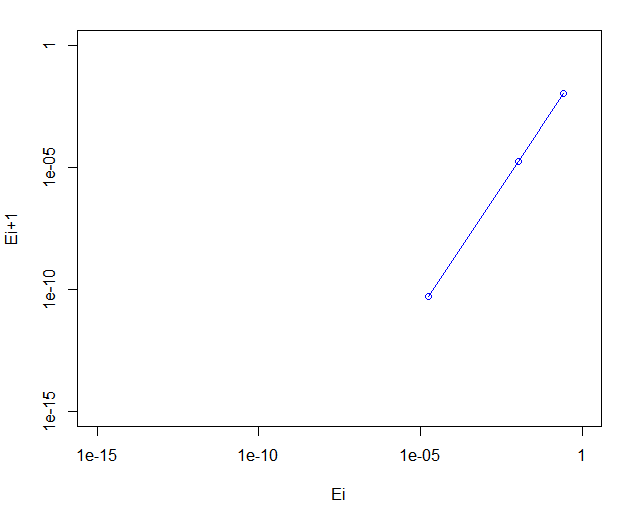
\includegraphics[scale=0.6]{img/relacion_error_aitken.png}
\vspace{-1em}
\caption{Relación entre $\varepsilon_i$ y $\varepsilon_{i+1}$ del del algoritmo $\Delta^2$ de Aitken}
\label{fig:relacion_error_aitken}
\end{figure}

\newpage

\subsection{Tolerancia contra Iteraciones}

A continuación se presenta la gráfica que modela la relación entre la cantidad de iteraciones que le toma al algoritmo obtener la raíz y el error calculado para esa iteración. El análisis se realizó a partir de la función $f(x)=cos^2(x)-x^2$ con punto inicial $x_0 = 1$. \par

% Figura: Tolerancia contra Iteraciones aitken
\vspace{-1em}
\begin{figure}[ht!]
\centering
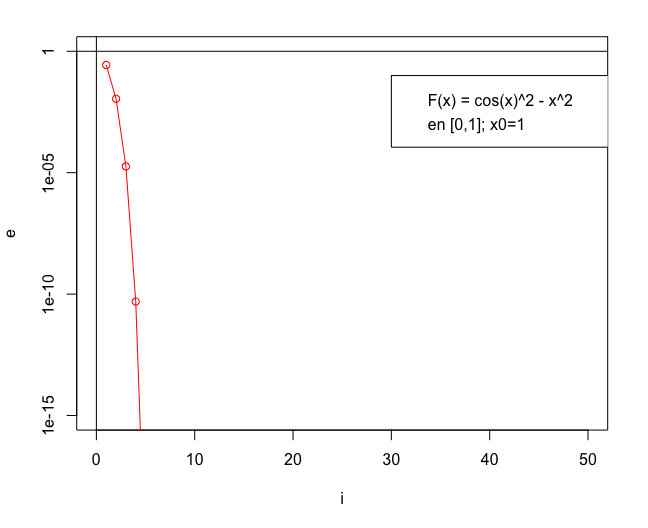
\includegraphics[scale=0.7]{img/tol_i_aitken.png}
\vspace{-1em}
\caption{Tolerancia vs. Iteraciones del algoritmo $\Delta^2$ de Aitken}
\label{fig:tol_i_aitken}
\end{figure}

\vspace{-1em}

\subsection{Comparación del Método contra el de Bisección}

Se estableció que el algoritmo $\Delta^2$ de Aitken es mucho más eficiente, alcanza una mayor tolerancia en mucho menor tiempo, y tiene menor pérdida de significancia a altas tolerancias. \par 

A continuación se presenta la gráfica que compara la convergencia del algoritmo $\Delta^2$ de Aitken contra el método de la bisección. El análisis se realizó a partir de la función $f(x)=cos^2(x)-x^2$ en el intervalo $[0,1]$ con punto inicial $x_0 = 1$. \par

% Figura: Aitken vs. Biseccion
\vspace{-1em}
\begin{figure}[ht!]
\centering
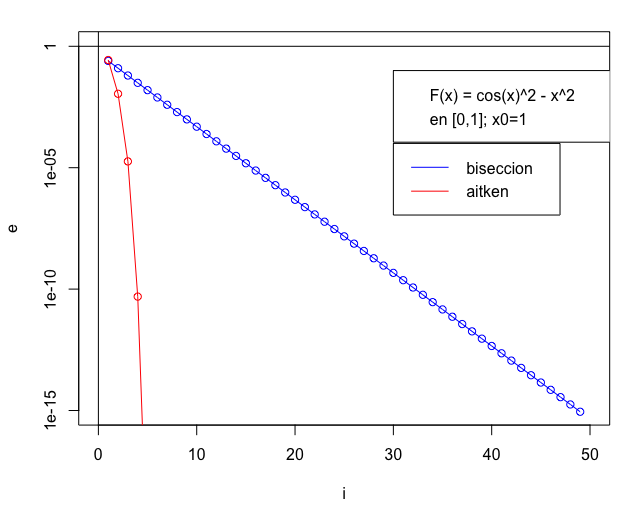
\includegraphics[scale=0.7]{img/aitken_vs_biseccion.png}
\vspace{-1em}
\caption{Algoritmo $\Delta^2$ de Aitken vs. Método de la Bisección}
\label{fig:aitken_biseccion}
\end{figure}

\newpage

\subsection{Comparación del Método contra Taylor}

La comparación entre el método con la solución por series de Taylor demostró que el algoritmo es mucho más preciso que una aproximación polinómica realizada mediante Taylor. \par 

El análisis se realizó para la función $f(x)=cos^2(x)-x^2$ con punto inicial $x_0 = 1$. La serie de Taylor se realizó centrada en $0$, de orden $16$. La herramienta para calcular la serie fue Wolfram Alpha. A continuación se presenta el polinomio obtenido: \par

\[ 1 - 2 x^2 + \frac{x^4}{3} - \frac{2x^6}{45} + \frac{x^8}{315} - \frac{2 x^{10}}{14175} + \frac{2 x^{12}}{467775} - \frac{4x^{14}}{42567525} + \frac{x^{16}}{638512875} + O(x^{18}) \]

La raíz correspondiente a este polinomio es: \par

\begin{table}[ht!]
\begin{tabular}{clc}
\multicolumn{1}{l}{} & \multicolumn{1}{c}{x}              & Tol                  \\
Taylor               & 0.73908513321519627015195351373908 &                      \\
Aitken               & 0.73908513321516064165531208767387 & 1.00E-32             \\
Valor Real           & 0.73908513321516064165531208767387 & \multicolumn{1}{l}{}
\end{tabular}
\end{table}

Como se puede evidenciar, comparando el valor obtenido mediante el método $\Delta^2$ de Aitken, se determina que el algoritmo es más preciso a la hora de calcular las soluciones.

\newpage

\end{document}

%%%%%%%%%%%%%%%%%%%%%%%%%%%%%%%%%%%%%%%%%%%%%%%%%%%%%%%%%%%%%%%%%%%%%%%
% Ejemplos
%%%%%%%%%%%%%%%%%%%%%%%%%%%%%%%%%%%%%%%%%%%%%%%%%%%%%%%%%%%%%%%%%%%%%%%

%%%%%%%%%%%%%%%%%%%%%%% Insertar Imágenes %%%%%%%%%%%%%%%%%%%%%%%%%%
%\begin{figure}[h!]
%\centering
%\includegraphics[scale=1.7]{img/ruta.jpg}
%\caption{Nombre de la figura}
%\label{fig:etiqueta}
%\end{figure}
